\documentclass[WordOneHalf]{XDUthesis} 

\title{基于压缩感知的大幅面太阳能组件缺陷检测技术}
\author{席若尧}
%\date{2015年12月02日}

%题目拆分:用于封面
\septitleA{基于压缩感知的大幅面}%如果论文题目长度<=11中文字符只需填此项即可B项空着
\septitleB{太阳能组件缺陷检测技术}%如果论文题目长度>11中文字符, 建议拆分为10+x or 11+x 将剩余x个字符填在此处。

\class{1316029}%班级号
\schoolnumber{13160299001}%学号
\major{空间科学与技术}%专业
\school{空间科学与技术}%学院
\supervisor{谢楷}%指导老师

% Avoid evil "This is unwritten. Stop BB and do it." image :)
\usepackage{todonotes}

% For the sake of some chemistry things...
\usepackage{chemformula}

\usepackage{subcaption}

\begin{document}

% 摘要
% 中文摘要
\begin{abstract}
本文介绍了太阳能电池的基本理论和工艺结构,描述了太阳能电池中的缺陷,总结了
传统的太阳能电池缺陷检测方法的优缺点;详细介绍了压缩感知理论;
介绍了近年来基于压缩
感知理论检测太阳能电池缺陷的新型方法,完成了基于压缩感知的太阳能电池缺陷
检测的数值仿真;介绍了现有的基于压缩感知的太阳能电池缺陷检测原型装置,及
其实现过程中遇到的困难。

针对太阳能电池栅状电极影响测量结果可压缩性,造成压缩感知检测方法的效率难以
进一步提高的问题,本文分别考虑栅状电极和实际的缺陷,将栅状电极视为对缺陷
分布图像的遮挡。通过光学成像获得栅状电极的遮挡区域,借鉴对于图像遮挡的修补
算法,对压缩感知的稀疏恢复算法进行改进,在求解过程中利用已知的遮挡区域信息,
同时修补图像遮挡,从而消除恢复结果中的栅状电极,增强结果的稀疏性,从而达到
降低采样次数,提高检测效率的目的。
\end{abstract}
\keywords{太阳能电池, 缺陷, 压缩感知, 稀疏性, 图像修补}

% 英文摘要
\begin{enabstract}
At first the basic theory, the processing and the structure of solar cells
are introduced.  The compressive sensing theory, and the new method to
detect solar cell defects with it are introduced in detail.  The numerical
emulation of this method is completed.  The existing prototypes detecting
solar cell defects with compressive sensing are introduced, and the
difficulties implementing them are discussed.

The fingers and busbars on the solar cells are affecting the sparsity of
solar cell defect image notably.  The time effiency of compressive
sensing method is limited by them.  To solve this issue, the fingers and
busbars and normal defects are considered seperately.  The fingers and
busbars are regarded as occlude areas of the defect image, and can be
acquiststioned with a optical camera.  Referencing the image inpainting,
the sparse signal recovery algorithms in compressive sensing are altered
to input the known occlude areas and inpaint them simutaniously.  The
result image without fingers and busbars are more sparse so the sampling
number could be reduced and the time effiency can be inproved.
\end{enabstract}
\enkeywords{solar cells, defects, compressive sensing, sparsity, image inpainting}


% 往PDF属性里面写下关键词信息
\makeatletter
\XDU@setpdf@keywords
\makeatother

\maketitle

% 文章主要部分

\chapter{引言}

Orz. \todo{dummy}

\chapter{基础理论}

% This chapter contains two sections irrevelant to each other.
% Seperate into two files.

\section{太阳能电池原理及结构简介}

目前,市售的太阳能电池以晶体硅太阳能电池为主。本节以晶体硅太阳能电池为例,
对太阳能电池的原理和结构进行介绍。

\subsection{太阳能电池的原理}

在抽象的意义下,晶体硅太阳能电池就是一个大的 p-n 结。当外界的光子流照射
晶体硅时,若光子的能量 $E = h\nu$ 不小于晶体硅的禁带宽度,则满带的电子就会
吸收该光子,并被激发到空带中。根据 Bloch 理论,空带中被激发出的少量电子可
以被视为自由电子,而满带中缺失的少量电子可以被视为带有正电荷的“空穴”。
对于普通的晶体硅,产生的电子-空穴对会以一定速率重新复合(即,被激发的电子
重新跃迁回满带,并辐射光子),电子-空穴对的产生率与复合率相等,没有宏观
电流。然而,由于 p-n 结耗尽区中存在极强的电场,在耗尽区中产生的电子和空穴
会在电场作用下向相反方向漂移,从而形成宏观的光电流。设 p-n 结的截面积是
$A$,耗尽区的宽度是 $W$,则光电流正比于单位时间内到达耗尽区内部的光子数:
\begin{equation} \label{eqn:LightCurrent}
I_L = K \cdot q_e L(W \cdot A)
\end{equation}
这里 $L$ 是光通量,$q_e$ 是电子的电荷量,$K$ 是和光的频率、半导体内部能带
结构等有关的常数。由于耗尽区很薄,$W$ 趋于 $0$ ,这里并不需要使用
Lambert-Beer 形式的吸收定律。

在太阳能电池不短路的情况下,光电流通过负载,将产生电压降 $V$。由于太阳能
电池本身是一个 p-n 结,在 $V$ 的偏置下,将产生电流:
\begin{equation} \label{eqn:Shockley}
I_F = I_S \left[ exp \left(\frac{q_e V}{k_B T} \right) - 1 \right]
\end{equation}
这就是Shockley 二极管方程,电流 $I_F$ 通常称为光电池的
暗电流。暗电流的方向与光电流 $I_L$ 相反,故总电流为:
\begin{equation} \label{eqn:TotalCurrent}
I = I_F - I_L
\end{equation}
短路时没有暗电流,故短路电流的大小和光电流相同:
\begin{equation} \label{eqn:SCCurrent}
I_{SC} = -I_L
\end{equation}

\subsection{晶体硅太阳能电池的内部结构}

晶体硅太阳能电池的 p-n 结是在厚度为 $200\mu m \sim 500\mu m$ 的 p 型硅晶体
上制作一 $0.2 \mu m \sim 0.5 \mu m$ 深的 n 型半导体层而成。 $n$ 层表面为
感光面,感光面用碱腐蚀成绒面,并喷涂一层减反射膜,以减小表面反射,提高
光电转化效率。

减反射膜下方印制主电极(busbar)和栅电极(finger),
主电极宽度约 $2mm$ ,栅电极宽度为
$0.1mm$,间距为 $3mm$ 。主电极和栅电极组成太阳能电池的负极。在这种设计
下,负极的总面积较小,减小了感光面积的损失。同时, $n$ 区的各个位置距离
栅电极都较近,有利于收集载流子,减少了载流子的复合损失。

在 p 衬底的下表面印制一层金属,作为正极,称为背电极。正负极和硅晶体之间
都形成良好的欧姆接触。整个太阳能电池的结构如图 \ref{fig:semantics} 所示。

\begin{figure}
\centering
\includegraphics[width=.8\textwidth]{Figure/semantics.pdf}
\caption{太阳能电池结构示意图}
\label{fig:semantics}
\end{figure}

\subsection{晶体硅太阳能电池的常见缺陷}

晶体硅太阳能电池中,任何组件的故障都可导致缺陷。下面简要介绍各种缺陷的成
因和形态。

\paragraph{固有缺陷} 是生产太阳能电池所用的硅材料本身的缺陷。理想状态下,
单晶硅是具有金刚石型晶胞的晶体,但这在现实中不可能。在加工过程中,杂质原子
会混入硅材料,同时由于温度、应力的不均,硅材料中将产生位错、层错、晶格空
位、间隙缺陷、 Frenkel 缺陷、 Schottky 缺陷等晶格缺陷。晶体缺陷将在很大
程度上影响局部的能带结构(甚至形成新的能级),可能提高载流子的复合率,导
致光子激发的电子-空穴对不能到达电极,从而形成低光电转化效率区域。

\paragraph{外部缺陷} 是在制造太阳能电池板的工艺过程中产生的,例如夹具和
量具在接触硅晶体时都可能导致表面污染,栅电极在印制过程中可能出现断线,
加工过程中电池板受到冲击可能出现裂纹,减反射膜可能过厚或过薄(均会影响
频率响应)。

图 \ref{fig:PLimage} 是采用 PL 法获得的一组缺陷图像,其中 a 是 \ch{Si3N4}
减反射膜上一处半椭圆形的缺损, b 是激光切割系统故障导致样品边缘出现的微
裂纹, c 是用螺旋测微计测量样品厚度时造成的表面污染, d 是硅片炉内退火时
温度不均产生的固有缺陷, e 是使用 RCA 标准清洗法处理硅片时夹具留下的痕迹,
f 是被严重污染的硅片\cite{FastPL}。

\begin{figure}
\centering
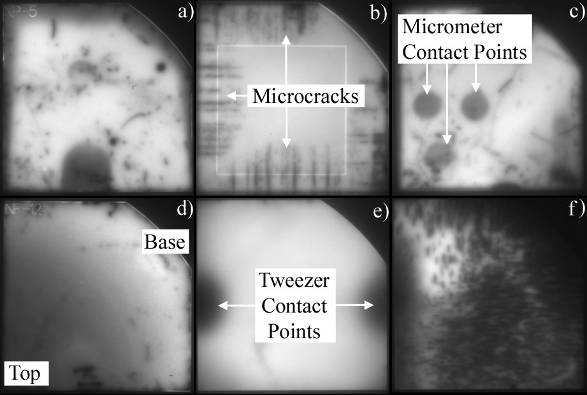
\includegraphics[width=.6\textwidth]{Figure/PLimage.png}
\caption{一些太阳能电池缺陷的 PL 图像}
\label{fig:PLimage}
\end{figure}

\section{压缩感知理论简介}

传统的图像采集遵循 Nyquist-Shannon 采样定理:
\begin{theorem}[采样定理] \label{th:Nyquist}
若函数 $x(t)$ 不含有频率高于 $B$ 的分量,则它可由在一列间距为 $1/(2B)$
的时间点上的采样值完全确定。
\end{theorem}

尽管定理 \ref{th:Nyquist} 的描述是针对时域采样,但对于空间域上的图像采集,
这一定理仍然适用。在日常生活中,如果用 CCD 相机等采样系统拍摄 LCD 显示器
等光栅系统,若采样系统的采样率过低,就会注意到 Moir\'e 条纹,这就
是欠采样导致的混叠。因此,现实中,人们往往尽量提高图像采集的采样率,以避
免发生混叠,保留图像中的细节信息。

然而,满足定理 \ref{th:Nyquist} 的采样往往导致过多的冗余测量值,占据巨大
的存储空间。另一方面,在某些特定应用中,满足定理 \ref{th:Nyquist} 的采样
会耗费过多的成本和时间。为此,人们开始探索新的采样理论,近年来形成的
压缩感知 (Compressive Sensing) 或称压缩采样
(Compressive Sampling) 理论就是一种重要的新型采样理论。

本文的太阳能电池缺陷检测方法以压缩感知作为理论基础,下面对其进行介绍。

\subsection{稀疏性和可压缩性}

CS 理论指出,可以从 $M (M << N)$ 个测量值中恢复包含 $N$ 个数据样本的信号
和图像。从信息论的视角来看,只有信号中包含的信息量比其带宽小得多时,才可能
达到这一目标。这一事实可由信号的稀疏性或可压缩性反映。

可用 $\ell_0$ 伪范数衡量离散信号(向量)的稀疏性:

\begin{definition}[$\ell_0$ 伪范数] \label{def:l0} 向量 $x$ 的
$\ell_0$ 伪范数定义为 $\mathbf{x}$ 中非零元素的个数:
\begin{equation}
\|x\|_0 = |\{k:x_k \neq 0\}|
\end{equation}
\end{definition}
注意定义 \ref{def:l0} 并不满足齐次性,因此不能称为范数或拟范数。

给定了稀疏性的衡量标准后,即可定义哪些向量是稀疏的。
\begin{definition}[$K$-稀疏] \label{def:K-sparse} 若
$\|x\|_0 \leq K$ ,则称 $x$ 是 $K$-稀疏 的。
称所有 $K$-稀疏信号组成的集合为 $\Sigma_K$。
\end{definition}

由于噪声的影响,实际信号不可能是严格稀疏的。但是,如果噪声不是特别强,
许多实际信号都可以通过稀疏信号近似表达。一般地,在信号 $x$ 中,选取
$K$ 个幅值最大的元素,将其余元素置为 $0$ ,即可得到该信号在 $\Sigma_K$
中最优的近似表达 $\hat x$\cite{KeepK}。 近似表达的误差可以用 $\ell_p$
范数定量衡量。
\begin{definition}[$\ell_p$ 范数, $\ell_p$ 拟范数] \label{def:lp}
\begin{equation}
\|x\|_p = \left( \sum x_k^p \right)^{\frac{1}{p}}
\end{equation}
若 $p \geq 1$ ,则 $\|x\|_p$ 满足三角不等式,称为 $\ell_p$ 范数。
若 $0 < p < 1$, $\|x\|_p$ 不满足三角不等式,称为 $\ell_p$ 拟范数。
\end{definition}

近似稀疏表达的误差一般用 $\ell_2$ 范数 $\|x - \hat x\|_2$ 加以衡量。信号
的近似稀疏表达早在压缩感知理论之前就被人们所熟知,并广泛用于
图像处理\cite{SparseImage}、信号压缩、统计学\cite{lasso}等领域。

尽管太阳能电池的缺陷图像并非传统意义上的光学图像,但是在工程实践中,人们仍
使用传统的图像压缩算法对太阳能电池缺陷图像进行压缩存储,且取得了较好的压缩
率。这表明,太阳能电池缺陷图像和光学图像一样,都存在较好的近似稀疏表达。

若给定数字图像的分辨率 $H \times W$ ,则该图像可以表示为长度为 $H \times W$
的向量 $x$ ,该向量由 $H$ 个长度为 $W$ 的向量 $r_1, r_1, \cdots, r_H$
连接而成,$r_k$ 表示图像的第 $k$ 行的 $W$ 个像素点。尽管在某些应用中将图像
表示为矩阵,但在 CS 理论中使用一维信号 $x$ 表示图像更为合适(这也是计
算机内存中二维数组的存储方式),因为 CS 理论本身并不关心信号的拓扑结构。

一般来说,表示图像的信号 $x$ 本身十分稠密。但是在合适的变换域中,该信号可能
被稀疏化。例如,若图像是水平、垂直方向的正弦波之积,那么 $x$ 不是稀疏的,但
其二维 Fourier 变换是 $1$-稀疏的。更一般地,可以将 $x$ 表示为 $T$ 个基本
波形,或称为原子的线性组合,即
\begin{equation}
x = \Phi a = \sum_{i=1}^T a_i \phi_i
\end{equation}
其中 $a_i$ 为 $x$ 在字典 $\Phi = [\phi_1, \phi_2, \cdots, \phi_T]$
下的稀疏表示系数;$\Phi$ 为 $N \times T$ 的矩阵,其列向量为原子 $\phi_k$。
若 $a = [a_1, a_2, \cdots a_T]$ 可用 $K$-稀疏 ($K << N$) 的系数向量
$\hat a$ 近似表示,且每个原子的 $\ell_2$ 范数 $\|\phi_k\|_2$ 相同(一般应
对字典作归一化),则可以只存储 $\hat a$ 中的 $K$ 个非零元素,并以线性组合
\begin{equation}
\hat x = \Phi \hat a
\end{equation}
较好地近似表示 $x$ 。

字典中原子的个数 $T$ 可能大于,等于,或者小于信号的长度 $N$ 。对于 Fourier
变换、 Hadamard 变换等正交变换,有 $T = N, \Phi^T = \Phi$ 。若 $T > N$ ,
则称 $a$ 是 $x$ 的过完备表示。 过完备表示看似浪费,但由于字典中的
原子更多,可以更好地匹配信号 $x$ 中的各种特征,因此往往能得到更稀疏的近似
表示。在许多实际情况下,必须使用过完备字典,才能得到较好的稀疏表示。

显然,过完备表示不是唯一的。为了找到最稀疏的过完备表示,需要求解下列优化
问题:
\begin{problem}[$\ell_0$ 优化问题]
\begin{equation}
\hat a = \mathop{\arg\min}_a \|a\|_0 \quad s.t. \quad \Phi a = x
\end{equation}
\end{problem}
对于有噪声的情况,松弛等式约束,得到:
\begin{problem}[稀疏逼近问题] \label{prob:SubsetOpt}
\begin{equation}
\hat a = \mathop{\arg\min}_a  \|a\|_0 \quad s.t. \quad \|x - \Phi a\|_2 < \epsilon
\end{equation}
\end{problem}
然而,问题 \ref{prob:SubsetOpt} 是一个 NP 难度问题 \cite{GJ79, SubsetOptNPC},
这类问题的高效精确求解是困扰计算机科学界多年的难题,我们不应贸然挑战这一
难题。为此,只能近似求解问题 \ref{prob:SubsetOpt} 。一种近似方法是,用具有
凸性的范数 $\ell_1$ 或 $\ell_2$ 代替 $\ell_0$ ,得到:
\begin{problem}[Lasso 回归问题] \label{prob:Lasso}
\begin{equation} \label{eqn:Lasso}
\hat a = \mathop{\arg\min}_a \|a\|_1 \quad s.t. \quad \|x - \Phi a\|_2 < \epsilon
\end{equation}
\end{problem}
\begin{problem}[岭回归问题] \label{prob:Ridge}
\begin{equation}
\hat a = \mathop{\arg\min}_a \|a\|_2 \quad s.t. \quad \|x - \Phi a\|_2 < \epsilon
\end{equation}
\end{problem}
实际上,求解问题 \ref{prob:Ridge} 并不能得到较为稀疏的解。这是由于
$\ell_2$ 球是一个超球,具有旋转不变性,其解一般不位于坐标轴上。但是对于
问题 \ref{prob:Lasso} 来说, $\ell_1$ 球是一个正轴形,其角位于坐标轴上。
在合理的约束条件下,问题 \ref{prob:Lasso} 的解将出现在正轴形的角上,这就
保证了解的稀疏性。

以上是对稀疏性和稀疏表示的基本介绍。图 \ref{Fig:Compress} 描述了利用稀疏表
示进行信号压缩的简要过程。

\begin{figure}
\centering
\fbox{
\begin{tikzpicture}[node distance=6cm]
\node (n0) {原始图像};
\node [right of=n0] (n1) {可压缩表示};
\node [right of=n1] (n2) {近似稀疏表示};
\draw[->] (n0.east) -- node [above] {正交变换} node [below] {或求解问题 \ref{prob:Lasso}} (n1);
\draw[->] (n1.east) -- node [above] {取 $K$ 个最大元素} (n2);
\end{tikzpicture}
} % fbox

\caption{信号压缩简要流程}
\label{Fig:Compress}
\end{figure}

在使用过完备表示的图像压缩算法中,我们通过求解问题 \ref{prob:Lasso} ,近似
求解了问题 \ref{prob:SubsetOpt},从而从 $N$ 个采样数据计算出 $T > N$ 个组合
系数 (即过完备表示)。如果我们可以进一步减少采样数据的个数至 $M < N < T$,
同时保证可以求解问题 \ref{prob:SubsetOpt} 而得到原图像的近似稀疏表示,
就能够降低采样的时间和设备成本。显然, $M$ 不能无限减小,
否则将导致问题 \ref{prob:SubsetOpt} 出现病态。
\begin{definition}[良定问题] \label{def:well-posed}
若一个优化问题存在唯一解,且该解在输入数据连续变化时也连续变化,则称该
优化问题在 Hadamard 意义下良定。
\end{definition}
\begin{definition}[病态问题] \label{def:ill-posed}
若一个优化问题的解不满足定义 \ref{def:well-posed} 要求的存在性、唯一性或者
连续性要求,则称该问题是病态 的 \cite{MathProblemImage}。
\end{definition}

另外,即使问题在数学上是良定的,在实际上,它的解可能并不是正确的过完备表示。
例如,若简单地随机选取 $M$ 个点进行采样,即有 $(N-M)$ 个缺失的采样点。这是
数字图像处理中经典的图像修补问题,其良定性早已得到证明\cite{inpainting}。
 然而,采样缺失部分的图像细节显然会丢失。

显然,只有对于特定的矩阵 $\Phi$ ,才能使得问题 $\ref{prob:Lasso}$ 良定,并
给出一个稀疏的 $\hat{a}$ ,使得 $\hat{x} = \Phi \hat{a}$ 是原图像的良好
近似。Cand\`es 和 Tao 等人对 $\Phi$ 必须满足的性质进行了研究,在稀疏表示
理论的基础上建立了压缩感知理论。

\subsection{感知矩阵 $\Phi$ 的特性}

一般来说,研究 $\Phi x = y$ 解集的性质,将从 $\Phi$ 的零空间 入手:
\begin{definition}[零空间]
矩阵 $\Phi$ 的零空间 定义为:
\begin{equation}
\mathcal{N}(\Phi) = \{z:\Phi z = 0\}
\end{equation}
即所有左乘 $\Phi$ 后得到零向量的向量组成的集合。
\end{definition}

对于任意稀疏信号 $a$ ,如果希望能够基于测量值 $y = \Phi a$ 唯一地重建 $a$,
则对于任意不同向量 $a_1, a_2 \in \Sigma_K$ ,
必有 $\Phi a_1 \neq \Phi a_2$,即:
\begin{equation}
\Phi (a_1 - a_2) \neq 0
\end{equation}
由于 $a_1 - a_2$ 可能是 $\Sigma_{2K}$ 中的任意非零向量,仅当
\begin{equation}
\Sigma_{2K} \cap \mathcal{N}(\Phi) = \{0\}
\end{equation}
时,即零空间 $\mathcal{N}(\Phi)$ 不包含非零的 $2K$-稀疏向量,
才能唯一地重建 $a$。

下面考虑非严格稀疏(可压缩)的向量。此时零空间不仅不能包含 $2K$-稀疏向量,
也不应
包含可以压缩的近似稀疏向量。设 $\Lambda \subset \{1, 2, \cdots, N\}$ 是
一组索引, $\Lambda^c = \{1,2,\cdots,N\} \backslash \Lambda$ 是其补集。
对于向量 $x$ 来说,我们保留其中下标属于 $\Lambda$ 的元素,而把下标属于
$\Lambda^c$ 的元素置为 $0$ 。据此,可以检验零空间内是否存在近似稀疏的
向量:
\begin{definition}[$K$ 阶零空间特性]
若存在常数 $C > 0$ ,使得对于所有 $h \in \mathcal{N}(\Phi)$ 和所有
$|\Lambda| \leq K$ 的 $\Lambda$ 都有
\begin{equation} \label{eq:NSP}
\|h_\Lambda\|_2 \leq C \frac{\|h_{\Lambda^c}\|_1}{\sqrt{K}}
\end{equation}
则称矩阵 $\Phi$ 满足 $K$ 阶零空间特性 (NSP)。
\end{definition}
NSP 的意义是,零空间中的向量 $h$ 的值并不集中在少数下标上。例如,若 $h$
是严格 $K$-稀疏的,则存在 $\Lambda$ 使得 $\|h_{\Lambda^c}\|_1 = 0$ 。
此时式 \ref{eq:NSP} 要求 $\|h_\Lambda\|_2 = 0$。因此,若 $A$ 满足 $K$
阶 NSP,则零空间 $\mathcal{N}(A)$ 中唯一的 $K$-稀疏向量是 $0$。

% 下列定理表明, NSP 是以较小误差成功恢复 $x$ 的必要条件:
% \begin{theorem} \label{th:NSP}
% 若 $\Delta:\mathbb{R}^{M} \rightarrow \mathbb{R}^T$ 是一个从 $M$ 个测量
% 恢复 $N$ 个系数 $a$ 的算法。若结果的误差由下式限定:
% \begin{equation}
% \|\Delta(\Phi x) - x\|_2  \leq  \frac{C}{\sqrt{K}}
% \min_{\hat x \in \Sigma_K}\|\hat x - x\|_1
% \end{equation}
% 则 $\Phi$ 满足 $2K$ 阶 NSP 。
% \end{theorem}
% \begin{proof}
% 假设 $h \in \mathcal{N}(\Phi)$,且 $\Lambda$ 是 $h$ 中最大的 $2K$ 个元素
% 的下标。将 $\Lambda$ 划分为 $\Lambda_0, \Lambda_1$, 使得
% $|\Lambda_1| = |\Lambda_2| = K$。令 $x = h_{\Lambda_1} + h_{\Lambda^c}$,
% $x' = -h_{\Lambda_0}$。由于 $x'$ 是严格 $K$-稀疏的,有 $\Delta(\Phi x')
% = x'$。注意到 $x - x' = h \in \mathcal{N}(\Phi)$ ,有:
% \begin{equation}
% Ah = A(x - x') = 0
% \end{equation}
% 即 $\Phi x' = \Phi x$ ,因此 $x' = \Delta(\Phi x)$。可知:
% \begin{equation}
% \|h_\Lambda\|_2 \leq \|h\|_2 = \|x - x'\|_2 = \|x - \Delta(\Phi x)\|_2
% \leq \frac{C}{\sqrt{K}} \min_{\hat x \in \Sigma_K} \|\hat x - x\|_1
% \leq \frac{\sqrt{2}C}{\sqrt{2K}} \|h_{\Lambda^c}\|_1
% \end{equation}
% \end{proof}
% 

NSP 保证了定义
\ref{def:well-posed} 中解的唯一性要求。然而,实际信号存在噪声和量化误差,
因此定义 \ref{def:well-posed} 还要求解的连续性。即,当输入 $y$ 发生微小
变化时,结果 $\hat a$ 应当也发生微小变化,而不应突变。这就要求更为严格的
重建条件。 Cand\`es 和 Tao 引入了下面的约束等距特性,
用以描述在有噪情况下稀疏信号可恢复的条件:
\begin{definition}[约束等距特性] 若存在 $\delta_k \in (0,1)$ ,使得:
\begin{equation}
(1 - \delta_K) \|a\|_2^2 \leq \|\Phi a\|_2^2 \leq (1 + \delta_K) \|a\|_2^2
\end{equation}
对所有 $a \in \Sigma_K$ 都成立,则称矩阵 $\Phi$ 满足 $K$ 阶约束等距
特性 (RIP)。使得 $\Phi$ 满足 $K$ 阶 RIP 的最小 $\delta_K$ 称为
$\Phi$ 的约束等距常数。
\end{definition}

若矩阵 $\Phi$ 满足 $2K$ 阶 RIP ,则对于任意 $a_1, a_2 \in \Sigma_K$,有:
\begin{equation}
(1 - \delta_K) \|a_1 - a_2\|_2^2 \leq \|\Phi a_1 - \Phi a_2\|_2^2
\leq (1 + \delta_K) \|a_1 - a_2\|_2^2
\end{equation}
若 $\delta_K$ 很小,则表明,任意两个 $K$-稀疏的向量经过 $\Phi$ 的线性变换
后,它们的欧几里得距离几乎不变。因此,若输入 $x = \Phi a$ 只受到微小扰动,
对应的 $a$ 也应只受到微小扰动。

实际上,RIP 比 NSP 更加严格。
\begin{theorem} \label{th:RIPimpliesESP}
若矩阵 $\Phi$ 满足 $\delta_K \leq \sqrt{2} - 1$ 时的 K 阶 RIP,则
$\Phi$ 必然满足 $2K$ 阶 NSP,且式 \ref{eq:NSP} 中的常数
\begin{equation}
C = \frac{\sqrt{2} \delta_{2K}}{1 - (1 + \sqrt{2}) \delta_{2K}}
\end{equation}
\end{theorem}

定理 \ref{th:RIPimpliesESP} 的详细证明非常复杂,超出了本文的范围,参见参考
文献 \cite{IntroCS}。

在 RIP 的基础上,Cand\`es 指出,问题 \ref{prob:Lasso} 的解是一个误差较小
的近似稀疏表示。
\begin{theorem} \label{th:l1recovery}
若感知矩阵 $\Phi$ 满足 $2K$ 阶 RIP,且约束等距系数 $\delta_{2K} < 
\sqrt{2} - 1$,且观测结果
\begin{equation} \label{eqn:observe}
y = \Phi a + z
\end{equation}
中的噪声 $z$ 满足 $\|z\|_2 \leq \epsilon$,则 Lasso 回归的结果
\begin{equation}
\hat a = \mathop{\arg\min}_{a'} \|a'\|_1 \quad s.t. \quad \|y-\Phi a'\|_2
\leq \epsilon
\end{equation}
满足
\begin{equation}
\|\hat a - a\|_2 \leq C_0 K^{-1/2} \|a - a_{\Lambda}\|_1 + C_1 \epsilon
\end{equation}
其中 $\Lambda$ 是 $a$ 中最大的 $K$ 个元素的下标集合,$C_0$ 和 $C_1$ 是
与 $\delta_{2K}$ 有关的较小的常数:
\begin{equation}
C_0 = 2 \times \frac{1 - (1-\sqrt{2}) \delta_{2K}}{1 - (1+\sqrt{2})
\delta_{2K}}, \quad C_1 = 4 \times \frac{\sqrt{1 + \delta_{2K}}}
{1 - (1 + \sqrt{2}) \delta_{2K}}
\end{equation}
\end{theorem}

定理 \ref{th:l1recovery} 的证明非常复杂,参见参考文献 \cite{RIPimplieCS}。
该定理从理论上表明了通过求解 Lasso 回归 (问题 \ref{prob:Lasso}),可以近似
地重构稀疏表示,且误差是有限的。

如果能够构造矩阵 $\Phi$ ,使其以约束等距常数 $\delta_{2K} < \sqrt{2}-1$
满足 $2K$ 阶 RIP ,即可用该矩阵作为压缩感知的感知矩阵。实践上,一般采用
随机方法构造矩阵 $\Phi$ 。具体地,将 $\Phi$ 分解为两个矩阵的乘积
\begin{equation}
y = \Phi a = H \Psi a = H x
\end{equation}
其中 $\Psi$ 是稀疏字典,以保证 $x$ 的稀疏性;而 $H$ 是一个 $M \times T$
的矩阵,其中 $T$ 是原子的个数, $M$ 是采样点数。在实际测量中,信号
$x = \Psi a$ 是物理上真实存在的信号,而 $H$ 是作用在物理信号 $x$ 上的测量,
称 $H$ 为测量矩阵。 已经证明,若 $x$ 足够
稀疏(稀疏度 $K$ 和 $M$ 相比足够小),字典 $\Psi$ 充分不相关,且 $H$ 是一个
随机矩阵,则 $\Phi = H \Psi$ 以高概率满足 $2K$ 阶 RIP 性质。因此,压缩感知
中的测量矩阵 $H$ 往往是随机矩阵。
\begin{definition}[相关性]
字典 $\Psi$ 的相关性 定义为:
\begin{equation}
\mu(\Psi) = \max_{i \neq j} \frac{|\psi_i^T \psi_j|}{\|\psi_i\|_2
\|\psi_j\|_2}
\end{equation}
即字典中任意两个不同原子(列向量)归一化内积绝对值的最大值。
\end{definition}

文献 \cite{CSRedundant} 证明了下列定理:
\begin{theorem} \label{th:RandomRIP}
若 $x \in \Sigma_K$ ,$2K \leq \mu(\Psi)^{-1}/16+1$ ,$H$ 是元素独立
同分布的随机矩阵,且采样点数 $M$ 足够大:
\begin{equation}
M \geq C_1(2K \log \frac{N}{2K} + 5.57 + t)
\end{equation}
其中 $C$ 是和 $H$ 的元素分布有关的常数,则 $\Phi = H \Psi$ 以概率
$1 - e^{-t}$ 满足 $\delta_{2K} \leq 1/3$ 的 $2K$ 阶 RIP。
\end{theorem}

由于 $1/3 < \sqrt{2} - 1$ ,该定理表明,矩阵 $\Phi$ 满足定理
\ref{th:l1recovery} 的要求,可以作为压缩感知的感知矩阵。另外, $t$ 在指数项
上,表明成功恢复的概率在理论门限附近迅速从 $0$ 增加到接近 $1$。

图 \ref{fig:CS} 描述了压缩感知的采样和稀疏恢复过程。

\begin{figure}
\centering
\fbox{
\begin{tikzpicture}[node distance=6cm]
\node (n0) {$x = \Psi a$};
\node [right of=n0] (n1) {$H\Psi a = \Phi a$};
\node [right of=n1] (n2) {$\hat a = \Delta(\Phi a)$};
\draw[->] (n0.east) -- node [above] {混叠欠采样} node [below] {测
量矩阵 $H$} (n1);
\draw[->] (n1.east) -- node [above] {稀疏恢复} node [below] {恢复算法
$\Delta$} (n2);
\end{tikzpicture}
} % fbox
\caption{压缩感知简要流程}
\label{fig:CS}
\end{figure}

我们已经讨论了感知矩阵 $\Phi$ 的性质。下面简要介绍常用的压缩感知稀疏
恢复算法。

\subsection{压缩感知中常用的稀疏恢复算法}

在压缩感知的框架下,测量值 $y$ 由式 \ref{eqn:observe} 给出,其中 $\Phi$
为感知矩阵, $z$ 为噪声。稀疏恢复算法的任务就是,根据给定的 $y$ 和 $\Phi$,
恢复出原始的稀疏信号 $x$。目前主流的稀疏恢复算法可分为凸优化类算法、贪心
算法、组合重建算法和贝叶斯算法这四类。下面简要介绍其中最为流行的凸优化类算
法和贪心算法。

在凸优化类算法中, $J(x)$ 是凸函数,且目标信号稀疏时, $J(x)$
的值较小。对于有噪声的测量值,为了重建稀疏信号 $x$ ,可以通过最小化 $J(x)$
促进 $x$ 的稀疏性,同时通过距离函数 $H$ 施加约束,使得 $\Phi x$ 接近测量值
$y$:
\begin{equation} \label{eqn:convexopt}
\hat x = \mathop{\arg \min}_{x'} J(x) \quad s.t. \quad H(\Phi x, y) \leq
\epsilon
\end{equation}
若选定 $J(x) = \|x\|_1$,$H(\Phi x, y) = \|\Phi x - y\|_2$,
则式 \ref{eqn:convexopt} 就成为式 \ref{eqn:Lasso},即 Lasso 回归问题
(问题 \ref{prob:Lasso})。该问题在数学和统计学上具有悠久的历史, Lasso
回归也是压缩感知领域非常重要的方法。在压缩感知领域, Lasso 回归又被称为
基追踪降噪 (BPDN) 问题。

对于图像来说,图像本身并不具有稀疏性,必须使用一稀疏字典 $\Psi$ 发掘其稀疏
性,才能通过 Lasso 或称 BPDN 求解。然而,在数字图像处理领域,往往可以假设
图像的梯度(即边缘)是稀疏的,并据此由测量值 $y$ 恢复 $x$。
\begin{definition} [全变分]
信号 $x$ 的全变分定义为:
\begin{equation}
TV(x) = \| |D(x)| \|_1
\end{equation}
即信号梯度的模的 $\ell_1$ 范数。
\end{definition}

根据之前对 $\ell_1$ 范数的讨论,最小化 $TV(x)$ 可以得到梯度稀疏的 $x$ 。
在式 \ref{eqn:convexopt} 中取 $J(x) = TV(x)$ ,即得到下列问题:
\begin{problem} \label{prob:TVopt}
\begin{equation}
\hat x = \mathop{\arg \min}_{x'} TV(x') \quad s.t. \quad 
\|\Phi x - y\|_2 \leq \epsilon
\end{equation}
\end{problem}
全变分最小化方法在核磁共振成像(MRI)领域的压缩感知问题中表现良好,这是由于
MRI 图像本身的梯度非常稀疏。然而,如果试图使用全变分最小化方法恢复梯度并不
稀疏的 $x$ ,将会产生强烈的伪迹。

凸优化是一个古老的研究课题,然而,已有的凸优化工具包往往并不适合压缩感知
问题。这是由于压缩感知中往往要面对高维信号,对优化求解的效率要求很高,
常规的优化算法无法满足压缩感知稀疏恢复的要求。例如,一般求解
\ref{prob:Lasso} 的方法是将其规约为二阶锥规划(SOCP) 问题,该问题
是现代优化方法研究的主要目标之一。但是,在压缩
感知稀疏恢复中,由于变量数和方程个数很大,SOCP 求解器运行十分缓慢。因此,
研究压缩感知的学者往往需要重新思考和开发新的优化算法。

贪心算法则采用完全不同的思路。 不同于求解巨大的全局优化问题,贪心算法在
每一步迭代中都选取目前看似最优的方案,期望通过局部最优解而产生全局最优解。

对于压缩感知中的稀疏信号恢复问题,最基本的贪心算法是匹配跟踪算法
(MP)。 在 MP 算法开始时,$x$ 的初步估计值 $x' = 0$,残差
$r = y - \Phi x'$从字典 $\Phi$ 中选取一个与 $y$ 相关性最大的列
$\phi_\lambda$ 。若相关系数为 $c$,就将组合系数 $x'_\lambda$ 增加 $c$,
同时残差将减小 $c \phi_\lambda$。反复执行这一步骤,直到残差的范数小于某个
预先设定的阈值,该算法终止。

在压缩感知的研究过程中, MP 算法被改进为正交匹配跟踪 (OMP)、逐步正交匹配
跟踪 (StOMP)、压缩感知匹配跟踪 (CoSaMP)、正则化正交匹配跟踪 (ROMP)、
等更加优秀的贪心算法。贪心算法的运行速度比全局凸优化快得多,然而抗噪声性能
很差,极少量的噪声就会导致恢复失败。因此,在实际应用中,往往只能使用
凸优化方法。


\chapter{系统理论设计和仿真}

本章利用前文描述的基础知识,对基于压缩感知的太阳能组件缺陷检测系统进行理论
设计和数值仿真。首先设计压缩感知系统的核心——测量矩阵 $\Phi$ ,之后以小波域
的 $\ell_1$ 范数优化(Lasso 回归)和空间域的全变分优化方法为例进行数值仿真
实验,以验证采用压缩感知方法检测太阳能组件缺陷的可行性。

\section{感知系统理论设计}

目前的压缩感知理论框架要求线性测量,非线性的稀疏恢复理论尚未成型。根据式
\ref{eqn:LightCurrent} 知道,光电流与面积 $A$ ,以及光通量 $L$ 成正比。
这说明,我们可以采用不同强度的光照射太阳能电池板感光面的各个不同位置,
总的光电流就是各个位置产生的光电流之和:
\begin{equation}
I_L = \sum_i I_i = \sum_i (W_i K_i)  L_i(q_e \cdot \delta A)
\end{equation}
这里 $\delta A$ 是小面积元的大小,而 $(W_i K_i)$ 衡量了位置 $i$ 的光电
转化效率。这个式子就相当于光电转化效率和 $L_i$ 的内积。进行多次测量,每次
采用一组不同的 $L_i$ 。于是, $L_i$ 就相当于测量矩阵 $H$ 中的行,
$I_L$ 就是 $y$ 中的一个采样点。

为了获得光电流的大小,我们需要采用输入阻抗趋于 $0$ 的互阻型放大器 (I-V
变换器)对太阳能电池的输出电流进行放大。此时太阳能电池几乎短路,根据式
\ref{eqn:SCCurrent} 知道,输出电流的大小等于光电流。如果放大器前级的输出
阻抗不接近 $0$ ,根据式 \ref{eqn:Shockley} 和 \ref{eqn:TotalCurrent} 知道,
测得的总电流和光电流之间存在指数关系,导致测量结果严重非线性,就不能应用
压缩感知理论。

注意到矩阵中的每一行相当于一组光通量,为简单起见,采用 Bernoulli 矩阵作为
测量矩阵 $H$ 。由于 Bernoulli 矩阵中各个元素相互独立,服从两点($0-1$)
分布,即使光电流与光通量并不严格线性,也不会导致无法恢复。

我们试用两种恢复算法对 $x$ 进行恢复。第一种方法是直接采用全变分最小化方法
(求解问题 \ref{prob:TVopt})恢复 $x$:
\begin{equation}
\hat x = \mathop{\arg\min}_{x'} TV(x') \quad s.t. \quad
\|Hx' - y\|_2 \leq \epsilon
\end{equation}

另一方面,考虑到某些缺陷的边界并不是非常尖锐,采用全变分最小化可能效果
不佳,尝试使用小波基 $\Psi$ 展示 $x$ 的稀疏性:
\begin{equation}
y = Hx = H\Psi a
\end{equation}
定义 $\Phi = H\Psi$,通过 Lasso 回归(求解问题 \ref{prob:Lasso})恢复
稀疏表示 $a$,进而恢复 $x$:
\begin{equation}
\hat x = \Psi \hat a = \Psi \mathop{\arg\min}_{a'} \|a'\|_1 \quad s.t.
\quad \|\Phi a' - y\|_2 \leq \epsilon
\end{equation}
注意到根据定理 \ref{th:RandomRIP},当 $H$ 的行数 $M$ 足够大时,矩阵 $\Phi$
以约束等距常数 $\delta_{2K} < 1/3$ 满足 $2K$ 阶 RIP。又根据定理
\ref{th:l1recovery} ,Lasso 回归能够以有限误差重构稀疏表示 $a$。

测量系统的框图如图 \ref{fig:system} 所示。

\begin{figure}
\centering
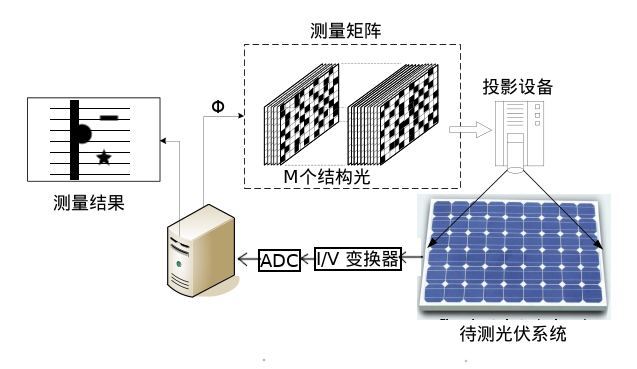
\includegraphics[width=.8\textwidth]{Figure/system.pdf}
\caption{测量系统框图}
\label{fig:system}
\end{figure}

下面我们将对这两种算法进行数值仿真,以比较它们的优劣。

\section{数值仿真}

\subsection{测试用例设计}

为了测试恢复算法的性能,需要设计一些具有代表性的测试用例。这里我们不深究
太阳能组件缺陷的产生原因,仅仅考虑缺陷的形态学特性。缺陷大致可以分为
坏点、裂纹和坏块,图 \ref{fig:testdata} 中的测试用例涵盖了这三种缺陷,
以及栅状电极的影响。

\begin{figure}
\centering
\begin{subfigure}[t]{1.1in}
	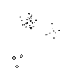
\includegraphics{Figure/testdata/0d.png}
	\caption{坏点}
	\label{fig:testdata:0d}
\end{subfigure}
\begin{subfigure}[t]{1.1in}
	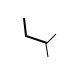
\includegraphics{Figure/testdata/1d.png}
	\caption{裂纹}
	\label{fig:testdata:1d}
\end{subfigure}
\begin{subfigure}[t]{1.1in}
	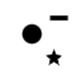
\includegraphics{Figure/testdata/2dsharp.png}
	\caption{边缘清晰的坏块}
\end{subfigure}
\begin{subfigure}[t]{1.1in}
	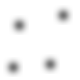
\includegraphics{Figure/testdata/2dsmooth.png}
	\caption{边缘模糊的坏块}
	\label{fig:testdata:2dsmooth}
\end{subfigure}
\begin{subfigure}[t]{1.1in}
	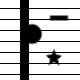
\includegraphics{Figure/testdata/2dsharp_finger.png}
	\caption{坏块与栅状电极}
\end{subfigure}
\caption{测试用例}
\label{fig:testdata}
\end{figure}

仿真中使用的随机矩阵 $H$ 为 Bernoulli 随机矩阵,其每一行均被标准化,使得
其 $\ell_2$ 范数为 $1$ ,均值为 $0$ 。这是多数压缩感知稀疏恢复算法对
测量矩阵的要求。 在实际测量中,我们不可能产生负的光通量,因此需要对采样数据
进行预处理,才能用恢复算法进行求解。

为了模拟实际测量时必然存在的噪声影响,我们为每组采样数据叠加 $10\%$ 的高斯
白噪声。由于 $H$ 的各行是归一化的,对采样数据增加噪声和对原始数据增加噪声
具有等价性。

$\ell1$ 最小化重建仿真中使用的小波基来自 \verb|ltfat| 软件包,其滤波器组为
$8$ 阶 Daubechies 滤波器,迭代次数为 $4$ 次\cite{ltfatnote015} 
\cite{ltfatnote030} 。

\subsection{全变分最小化重建的仿真结果}

全变分最小化重建均使用 Li 编写的 \verb|TVAL3| 软件包完成。该软件包
采用增广拉格朗日乘子法和交替方向算法求解全变分最小化重建问题,是一款非常
优秀的全变分最小化求解器。关于该软件包的设计思路和实现细节,参见文献
\cite{TVAL3CBLMaster} \cite{TVAL3CBLPhD}。

对坏点(图 \ref{fig:testdata:0d} )的重建结果如图 \ref{fig:TV0d} 所示。

\begin{figure}
\centering
\begin{subfigure}[t]{1.1in}
	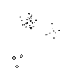
\includegraphics{Figure/testdata/0d.png}
	\caption{原始数据}
\end{subfigure}
\begin{subfigure}[t]{1.1in}
	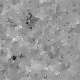
\includegraphics{Figure/TV/0d10.png}
	\caption{$M = 0.1 N$}
\end{subfigure}
\begin{subfigure}[t]{1.1in}
	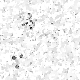
\includegraphics{Figure/TV/0d30.png}
	\caption{$M = 0.3 N$}
\end{subfigure}
\begin{subfigure}[t]{1.1in}
	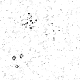
\includegraphics{Figure/TV/0d50.png}
	\caption{$M = 0.5 N$}
\end{subfigure}
\begin{subfigure}[t]{1.1in}
	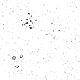
\includegraphics{Figure/TV/0d70.png}
	\caption{$M = 0.7 N$}
\end{subfigure}
\caption{坏点的全变分最小化重建结果}
\label{fig:TV0d}
\end{figure}

可见, $M = 0.1 N$ 时重建完全失败,这是由于 $M$ 太小,不满足定理
\ref{th:RandomRIP} 的要求,导致矩阵 $H$ 丧失 RIP 性质。

对裂纹(图 \ref{fig:testdata:1d} )的重建结果如图 \ref{fig:TV1d} 所示。

\begin{figure}
\centering
\begin{subfigure}[t]{1.1in}
	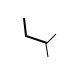
\includegraphics{Figure/testdata/1d.png}
	\caption{原始数据}
\end{subfigure}
\begin{subfigure}[t]{1.1in}
	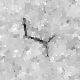
\includegraphics{Figure/TV/1d10.png}
	\caption{$M = 0.1 N$}
\end{subfigure}
\begin{subfigure}[t]{1.1in}
	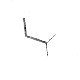
\includegraphics{Figure/TV/1d30.png}
	\caption{$M = 0.3 N$}
\end{subfigure}
\begin{subfigure}[t]{1.1in}
	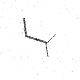
\includegraphics{Figure/TV/1d50.png}
	\caption{$M = 0.5 N$}
\end{subfigure}
\begin{subfigure}[t]{1.1in}
	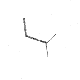
\includegraphics{Figure/TV/1d70.png}
	\caption{$M = 0.7 N$}
\end{subfigure}
\caption{裂纹的全变分最小化重建结果}
\label{fig:TV1d}
\end{figure}

除了 $M = 0.1N$ 时重建结果很差外,其他三次重建都较好地恢复了
图像中的裂纹。然而,可以注意到裂纹出现较为明显的锯齿,这是由于
全变分最小化会促进图像梯度的稀疏性,导致图像出现类似阶梯函数的
特性。

对边界清晰的坏块重建结果见图 \ref{fig:TV2dsharp}。
可以看出,全变分最小化对边界稀疏的图像重建效果很好,甚至只要
$10\%$ 的采样即可几乎完美地恢复出图像中的三个坏块。

\begin{figure}
\centering
\begin{subfigure}[t]{1.1in}
	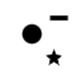
\includegraphics{Figure/testdata/2dsharp.png}
	\caption{原始数据}
\end{subfigure}
\begin{subfigure}[t]{1.1in}
	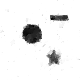
\includegraphics{Figure/TV/2dsharp10.png}
	\caption{$M = 0.1 N$}
\end{subfigure}
\begin{subfigure}[t]{1.1in}
	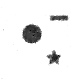
\includegraphics{Figure/TV/2dsharp30.png}
	\caption{$M = 0.3 N$}
\end{subfigure}
\begin{subfigure}[t]{1.1in}
	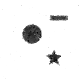
\includegraphics{Figure/TV/2dsharp50.png}
	\caption{$M = 0.5 N$}
\end{subfigure}
\begin{subfigure}[t]{1.1in}
	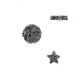
\includegraphics{Figure/TV/2dsharp70.png}
	\caption{$M = 0.7 N$}
\end{subfigure}
\caption{边界清晰坏块的全变分最小化重建结果}
\label{fig:TV2dsharp}
\end{figure}

对边界模糊的坏块重建结果如图 \ref{fig:TV2dsmooth}
所示。重建结果很差,这是由于图像
\ref{fig:testdata:2dsmooth} 的梯度并不十分稀疏,导致定理
\ref{th:RandomRIP} 的条件难以满足。可见,全变分最小化方法不适合
恢复颜色变化较为平滑的图像。

\begin{figure}
\centering
\begin{subfigure}[t]{1.1in}
	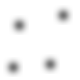
\includegraphics{Figure/testdata/2dsmooth.png}
	\caption{原始数据}
\end{subfigure}
\begin{subfigure}[t]{1.1in}
	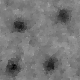
\includegraphics{Figure/TV/2dsmooth10.png}
	\caption{$M = 0.1 N$}
\end{subfigure}
\begin{subfigure}[t]{1.1in}
	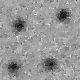
\includegraphics{Figure/TV/2dsmooth30.png}
	\caption{$M = 0.3 N$}
\end{subfigure}
\begin{subfigure}[t]{1.1in}
	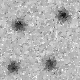
\includegraphics{Figure/TV/2dsmooth50.png}
	\caption{$M = 0.5 N$}
\end{subfigure}
\begin{subfigure}[t]{1.1in}
	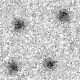
\includegraphics{Figure/TV/2dsmooth70.png}
	\caption{$M = 0.7 N$}
\end{subfigure}
\caption{边界模糊坏块的全变分最小化重建结果}
\label{fig:TV2dsmooth}
\end{figure}

对栅状电极的重建结果如图 \ref{fig:TVfinger}
所示。可以看出,栅状电极的存在严重破坏了梯度的稀疏性,导致
全变分最小化恢复过程需要更多的采样数据。

\begin{figure}
\centering
\begin{subfigure}[t]{1.1in}
	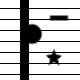
\includegraphics{Figure/testdata/2dsharp_finger.png}
	\caption{原始数据}
\end{subfigure}
\begin{subfigure}[t]{1.1in}
	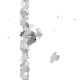
\includegraphics{Figure/TV/finger10.png}
	\caption{$M = 0.1 N$}
\end{subfigure}
\begin{subfigure}[t]{1.1in}
	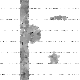
\includegraphics{Figure/TV/finger30.png}
	\caption{$M = 0.3 N$}
\end{subfigure}
\begin{subfigure}[t]{1.1in}
	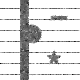
\includegraphics{Figure/TV/finger50.png}
	\caption{$M = 0.5 N$}
\end{subfigure}
\begin{subfigure}[t]{1.1in}
	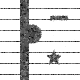
\includegraphics{Figure/TV/finger70.png}
	\caption{$M = 0.7 N$}
\end{subfigure}
\caption{坏块与栅状电极的全变分最小化重建结果}
\label{fig:TVfinger}
\end{figure}

\subsection{$\ell_1$ 范数最小化重建的仿真结果}

$\ell_1$ 范数最小化重建采用 Zhang 等编写的 \verb|YALL1| 软件包完成。该
软件包功能强大,可求解多种形式的 $\ell_1$ 优化问题。和 \verb|TVAL3| 一样,
该软件包也采用交替方向算法进行最优化求解,运行效率较高,能够高效地完成
数值仿真。

图 \ref{fig:l10d} 给出了坏点仿真数据(图 
\ref{fig:testdata:0d} )的 $\ell_1$ 最小化恢复结果。

\begin{figure}
\centering
\begin{subfigure}[t]{1.1in}
	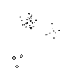
\includegraphics{Figure/testdata/0d.png}
	\caption{原始数据}
\end{subfigure}
\begin{subfigure}[t]{1.1in}
	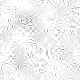
\includegraphics{Figure/L1/0d10.png}
	\caption{$M = 0.1 N$}
\end{subfigure}
\begin{subfigure}[t]{1.1in}
	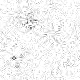
\includegraphics{Figure/L1/0d30.png}
	\caption{$M = 0.3 N$}
\end{subfigure}
\begin{subfigure}[t]{1.1in}
	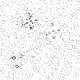
\includegraphics{Figure/L1/0d50.png}
	\caption{$M = 0.5 N$}
\end{subfigure}
\begin{subfigure}[t]{1.1in}
	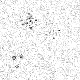
\includegraphics{Figure/L1/0d70.png}
	\caption{$M = 0.7 N$}
\end{subfigure}
\caption{坏点的 $\ell_1$ 最小化重建结果}
\label{fig:l10d}
\end{figure}

可见, $M = 0.1 N$ 时重建仍然完全失败。由于小波变换并不能增加坏点图像的
稀疏性,此时测量矩阵 $\Phi = H \Psi$ 同全变分最小化求解时使用的矩阵 $H$
一样,不满足 RIP 条件。因此,$M = 0.1N$ 时,无论采用何种算法,只要无法
在某个字典下稀疏表示坏点,都几乎不可能成功重建图像。

$M$ 较大时则可以成功重建图像,但是注意到 $M=0.7$ 时的重建结果中,噪点比
$M=0.5$ 时更多,直观上图像质量发生了退化。这是由于 $\Phi$ 规模的增加
加强了 Lasso 回归的约束条件:
\begin{equation}
\|\Phi a' - y\|_2 \leq \epsilon
\end{equation}
从而降低了 $\ell_1$ 优化的自由度,导致 $\ell_1$ 最小化本身具有的降噪功能
难以充分发挥。

图 \ref{fig:L11d} 给出针对裂纹的测试数据(图 \ref{fig:testdata:1d} )
的重建结果。

\begin{figure}
\centering
\begin{subfigure}[t]{1.1in}
	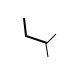
\includegraphics{Figure/testdata/1d.png}
	\caption{原始数据}
\end{subfigure}
\begin{subfigure}[t]{1.1in}
	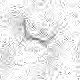
\includegraphics{Figure/L1/1d10.png}
	\caption{$M = 0.1 N$}
\end{subfigure}
\begin{subfigure}[t]{1.1in}
	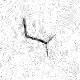
\includegraphics{Figure/L1/1d30.png}
	\caption{$M = 0.3 N$}
\end{subfigure}
\begin{subfigure}[t]{1.1in}
	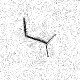
\includegraphics{Figure/L1/1d50.png}
	\caption{$M = 0.5 N$}
\end{subfigure}
\begin{subfigure}[t]{1.1in}
	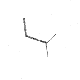
\includegraphics{Figure/TV/1d70.png}
	\caption{$M = 0.7 N$}
\end{subfigure}
\caption{裂纹的 $\ell_1$ 最小化重建结果}
\label{fig:L11d}
\end{figure}

除了 $M = 0.1N$ 时重建结果很差外,其他三次重建都较好地恢复了
图像中的裂纹。

对边界清晰的坏块重建结果见图 \ref{fig:L12dsharp}。
可以看出,边界稀疏图像更适合采用全变分最小化恢复, $\ell_1$ 恢复
求解的结果在 $M$ 较小时较全变分方法更差。

\begin{figure}
\centering
\begin{subfigure}[t]{1.1in}
	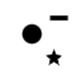
\includegraphics{Figure/testdata/2dsharp.png}
	\caption{原始数据}
\end{subfigure}
\begin{subfigure}[t]{1.1in}
	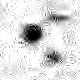
\includegraphics{Figure/L1/2dsharp10.png}
	\caption{$M = 0.1 N$}
\end{subfigure}
\begin{subfigure}[t]{1.1in}
	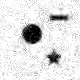
\includegraphics{Figure/L1/2dsharp30.png}
	\caption{$M = 0.3 N$}
\end{subfigure}
\begin{subfigure}[t]{1.1in}
	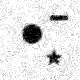
\includegraphics{Figure/L1/2dsharp50.png}
	\caption{$M = 0.5 N$}
\end{subfigure}
\begin{subfigure}[t]{1.1in}
	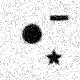
\includegraphics{Figure/L1/2dsharp70.png}
	\caption{$M = 0.7 N$}
\end{subfigure}
\caption{边界清晰坏块的 $\ell_1$ 最小化重建结果}
\label{fig:L12dsharp}
\end{figure}

对边界模糊的坏块重建结果如图 \ref{fig:L12dsmooth}
所示。重建结果与全变分最小化的结果相比较好,因为小波变换相比于求梯度能更好
地增加该图像的稀疏性。然而,横向比较表明,重建结果仍然不如其他测试数据,说
明仍需进行进一步研究,寻找能够稀疏表示边界模糊坏块的字典。

\begin{figure}
\centering
\begin{subfigure}[t]{1.1in}
	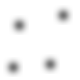
\includegraphics{Figure/testdata/2dsmooth.png}
	\caption{原始数据}
\end{subfigure}
\begin{subfigure}[t]{1.1in}
	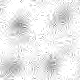
\includegraphics{Figure/L1/2dsmooth10.png}
	\caption{$M = 0.1 N$}
\end{subfigure}
\begin{subfigure}[t]{1.1in}
	\includegraphics{Figure/L1/2dsmooth30.png}
	\caption{$M = 0.3 N$}
\end{subfigure}
\begin{subfigure}[t]{1.1in}
	\includegraphics{Figure/L1/2dsmooth50.png}
	\caption{$M = 0.5 N$}
\end{subfigure}
\begin{subfigure}[t]{1.1in}
	\includegraphics{Figure/L1/2dsmooth70.png}
	\caption{$M = 0.7 N$}
\end{subfigure}
\caption{边界模糊坏块的 $\ell_1$ 最小化重建结果}
\label{fig:L12dsmooth}
\end{figure}

对栅状电极的重建结果如图 \ref{fig:L1finger}
所示。 栅状电极的存在也严重破坏了图像在小波字典下的稀疏性,直到 $M = 0.5N$
时才能够较好地恢复图像。

\begin{figure}
\centering
\begin{subfigure}[t]{1.1in}
	\includegraphics{Figure/testdata/2dsharp_finger.png}
	\caption{原始数据}
\end{subfigure}
\begin{subfigure}[t]{1.1in}
	\includegraphics{Figure/L1/finger10.png}
	\caption{$M = 0.1 N$}
\end{subfigure}
\begin{subfigure}[t]{1.1in}
	\includegraphics{Figure/L1/finger30.png}
	\caption{$M = 0.3 N$}
\end{subfigure}
\begin{subfigure}[t]{1.1in}
	\includegraphics{Figure/L1/finger50.png}
	\caption{$M = 0.5 N$}
\end{subfigure}
\begin{subfigure}[t]{1.1in}
	\includegraphics{Figure/L1/finger70.png}
	\caption{$M = 0.7 N$}
\end{subfigure}
\caption{坏块与栅状电极的 $\ell_1$ 最小化重建结果}
\label{fig:L1finger}
\end{figure}

以上仿真结果表明,压缩感知方法确实可以检测太阳能电池中的缺陷,且采样次数
为对整个光学面采样的 $10\%$ 至 $50\%$ 。仿真结果是在较为理想的情况下得出的,
在实际工作中,文献 \cite{XDUCLBIC} 建议使用 $40\%$ 至 $60\%$ 的采样次数,
而文献 \cite{CLBIC17} 建议使用 $40\%$ 至 $80\%$。

\chapter{现有压缩感知缺陷检测原型分析}

目前,英国国家物理实验室 (NPL) 团队和西安电子科技大学团队分别独立完成了
基于压缩感知的太阳能电池缺陷检测装置原型。本章讨论这两套装置的设计和实现,
说明压缩感知方法在实际应用时遇到的一些问题。

\section{NPL 的原型装置}

NPL 自 2014 年起开始构建其基于压缩感知的太阳能缺陷检测装置原型。该装置的
光源为一激光二极管,其产生的 $636.2 nm$ 激光照射在一数字微镜器件 (DMD)
上。DMD 光学面上的大量微小镜面由外部提供的信号驱动,产生对应的结构光。
为了消除 DMD 产生的衍射效应,采用空间频率滤波器过滤结构光,
用过滤后的结构光照射被测太阳能电池。产生的光电流经 I-V
变换和采样后得到一次测量的结果。

NPL 装置采用一种称为 SBHE 的测量矩阵 \cite{BlockHadamard} :
\begin{definition}[SBHE 矩阵]
\begin{equation}
\Phi = Q_M W P_N
\end{equation}
其中
\begin{equation}
W = diag\{W_B, W_B, \cdots, W_B\}
\end{equation}
$W_B$ 是 $B \times B$ 的 Hadamard 矩阵,$P_N$ 是一个随机的置换矩阵,
$Q_M$ 是一个随机的 $M \times N$ 矩阵,选取 $W P_N$ 的 $M$ 行。
\end{definition}

和完全随机的测量矩阵相比,SBHE 的突出优点是计算复杂度较小。置换
$P_N$ 只需要 $O(N)$ ,$Q_M$ 的作用是选取 $M$ 行,只需要 $O(M)$ ,而
$W$ 相当于 $N/B$ 次快速 Hadamard-Walsh 变换,时间复杂度为
\begin{equation}
T(N,B) = O(N + M + N/B \times B log B) = O(N(1+logB))
\end{equation}
相比于完全随机矩阵需要 $O(NM)$ 的运算时间,SBHE 的运算速度要快得多,可以
有效减少重建时间。和 Bernoulli 矩阵一样, SBHE 是二值化的,因此容易在光学
系统中实现。实践表明,一般选取 $B=32$ 就能得到较好的效果。

\section{西安电子科技大学的原型装置}

和 NPL 的实现相比,西安电子科技大学团队的原型装置是在较短时间内完成的,
其结构也较为简单。作为研究原型,它没有使用 DMD ,而是直接将待测太阳能电池
贴在 LCD 显示器上,由显示器提供结构光。这种方法成本较低,但不能适用于更大
的太阳能组件。另外,由于没有使用激光光源,结构光的光谱并不匹配太阳能电池
的最大响应波段,这些问题需要在后续实验中进行改进。

文献 \cite{XDUCLBIC} 指出,该装置相比于传统的 LBIC 扫描法,时间效率有
$10$ 至 $15$ 倍的提升。实际上,时间效率的提升是两种因素的共同作用。首先,
该装置使用 LCD 作为光源,避免了机械运动环节,极大地提升了测量效率。例如,
对于某一特定太阳能电池, LBIC 需要对 $6400$ 个测试点依次扫描,消耗时间为
$1280 s$ 左右。而 CLBIC 系统即使在测量 $6400$ 个光电流数据的情况下,测量
过程和图像重建过程的总时间
也仅有 $170 s$,相当于时间效率提高 $7$ 倍。其次,根据压缩感知理论, CLBIC
系统对光电流的测量次数比 LBIC 少。例如,如果将测量次数减少到测试点个数的
$30\%$ ,即 $1920$ 次,则 CLBIC 的总耗时进一步减小到 $87 s$ ,时间效率相比
进行 $6400$ 次采样时又提升 $1$ 倍,相比于 LBIC 方法提升 $15$ 倍。

理论上,我们当然可以用 LCD 代替机械扫描装置,在每次测量时只点亮 LCD 的一个
测试点,从而直接得到太阳能电池的缺陷分布。然而,实际上,由于没有聚焦装置,
这种方法浪费了 LCD 光源的绝大多数能量,导致信噪比大幅下降,实践中根本不足
取。而压缩感知方法则不然,在压缩感知的测量中,每次均有约一半的光源能量被
利用。因此,尽管 LCD 引起的效率提升看上去和压缩感知无关,实际上却只有压缩
感知方法才能直接使用 LCD 作为光源,从而避免聚焦和机械扫描。

\section{原型装置遇到的问题}

在实验过程中,两个原型装置遇到了一些共同的问题。

(1) 太阳能电池的栅状电极破坏了测量结果的稀疏性,正如在仿真中发现的一样,
栅状电极的存在导致我们要增加 $20\%$ 至 $40\%$ 的测量,提高了测量和恢复需要
的时间。

(2) 在采样次数接近 $90\%$ 的时候,从理论上讲,应该得到非常好的恢复结果。
然而,两个团队都发现,由于噪声的存在,当采样次数较大时,根本无法得到有意义
的恢复结果。进一步的分析表明,造成这一现象的噪声作用于测量矩阵,而非采样
结果本身,压缩感知恢复算法的抗噪能力对矩阵噪声不能发挥作用。

(3) 随着问题规模的提高,恢复算法的运算量以立方级别增加。如果要在工业上
使用压缩感知方法检测太阳能缺陷,势必遇到运算量过大的问题。对此,两个团队
都建议,可以使用云计算、 FPGA 等高并发的编程平台来缓解这一问题,并应对
恢复算法进行改进和优化,以减小计算量。

\chapter{光学成像辅助的压缩感知缺陷检测}

\section{问题描述}

文献 \cite{XDUCLBIC} 指出,在基于压缩感知的缺陷检测系统中,太阳能电池表面
栅状电极覆盖的区域的光电转化效率为 $0$ 。这些线状区域的存在严重破坏了信号
的稀疏性。对于全变分最小化方法,求梯度完全不能降低线状目标的稀疏性;
对于 $\ell_1$ 最小化方法,必须寻找一个能够稀疏表示直线的字典,才能降低
栅状电极的稀疏性。目前确实有这样的字典存在,即脊波(Ridgelet)
和曲波(Curvelet)变换\cite{ridgelet} \cite{curvelet} 。 十分巧合的
是,这两种变换正是由压缩感知理论的提出者 Cand\`es 和 Donoho 发明的。
然而,脊波和曲波变换的数学形式较为复杂,程序运行较慢,对于迭代次数较多的
优化问题而言,会极大增加优化算法的运行时间。

本文采用另一种方案,解决栅状电极带来的稀疏性退化问题。由于栅状电极在光学
上是可见的,我们可以用光学相机获取栅状电极的位置。从信息论的角度出发,当
我们获得了栅状电极的位置信息后,如果我们能够合理地运用这些信息,就可能
减少压缩采样过程需要获取的信息量,从而减少采样次数,提高检测效率。本章
的后续内容将表明,这的确是可行的。

\section{数学模型}

考虑问题的物理本质,栅状电极覆盖区域的光电转化效率为 $0$ ,纯粹是由于它
被电极覆盖的缘故,与电极之下的硅材料毫无关系。假如栅状电极是透明的(现实中
并没有这样良好的电极材料),它对测量结果没有影响,得到的测量结果是稀疏的。
然而,由于栅状电极的遮挡,被遮挡区域的测量值直接变为 $0$ ,导致稀疏
性退化。这样,自然想到采用图像修补算法,去除图像上的遮挡,尽可能
恢复未被遮挡的,稀疏的图像,从而提高压缩感知的效率和准确性。

下面给出图像修补问题的数学描述:
\begin{problem}[图像修补]
设有一矩阵 $H = diag\{W\}$,$W \in \{0,1\}^{N}$。设 $x$ 是一维向量
化的图像,则被遮挡并有噪声 $z$ 污染的图像为
\begin{equation}
y = Hx + z
\end{equation}
已知 $y$ 和 $H$ ,恢复未被遮挡的图像 $x$。
\end{problem}

和压缩感知恢复问题一样,图像修补问题亦可通过求解全变分最小化或 $\ell_1$
最小化解决,下面以全变分最小化为例说明。
\begin{equation}
\hat x = \mathop{\arg\min}_{x'} TV(x') \quad s.t. \quad
\|Hx' - y\|_2 \leq \epsilon
\end{equation}
注意虽然图像修补问题和压缩感知恢复问题都能够用全变分最小化方法求解,但其
内涵截然不同。在压缩感知理论中,若矩阵 $H$ 满足 RIP ,则可以认为测量
结果包含足够信息,因此能够以有限误差恢复 $x$ 。然而,在图像修补问题中,矩阵
$H$ 连 NSP 都不满足,更不会满足 RIP 。从信息论的角度来说,图像中被遮挡部分
的信息已经完全丢失,只能通过其他位置的信息,结合实际图像梯度稀疏的性质,采
用全变分最小化推测被遮挡部分的值。图 \ref{fig:BarbaraMask} 是在著名的
Barbara 图像上模拟遮挡栅状电极后的恢复结果,可以看出其中的直线状模糊痕迹,
即为被遮挡的部分。

\begin{figure}
\centering
\begin{subfigure}[t]{1.5in}
\includegraphics[width=1.5in]{Figure/barbara.png}
\caption{原始图像}
\end{subfigure}
\begin{subfigure}[t]{1.5in}
\includegraphics[width=1.5in]{Figure/barbara_mask.png}
\caption{被遮挡的图像}
\end{subfigure}
\begin{subfigure}[t]{1.5in}
\includegraphics[width=1.5in]{Figure/barbara_out.png}
\caption{恢复的图像}
\end{subfigure}
\caption{Barbara 图像的遮挡和恢复结果}
\label{fig:BarbaraMask}
\end{figure}

尽管如此,我们仍可以借鉴图像修补问题的思想,用于压缩感知问题。我们称图像修补
问题的遮挡矩阵为 $H_1$ ,压缩采样的测量矩阵为 $H_2$。对于图像修补,求解全
变分最小化问题可以恢复原图像,直观地看,这是由于 $H_1$ 的零空间包含被遮挡的
点,优化算法可以自由改变它们的值,以达到减小全变分的目的。同样的,在我们的
压缩感知理论中,鉴于无法确定被遮挡的值,同样应该将这些点加入零空间,使其
可以自由变化。为了达到这一目的,采用矩阵
\begin{equation}
H = H_2 H_1
\end{equation}
作为新的测量矩阵。其中,$H_1$ 的零空间包含所有被遮挡的像素点,赋予了优化算
法足够的自由度,可以通过调整这些点的值尽量降低全变分,使它们不对最终的目标
函数产生较大影响。 $H_2$ 则满足 RIP ,因此其不涉及被遮挡点的子矩阵同样满足
RIP,使得未被遮挡的像素点能够稳定、准确地被恢复。

\section{系统仿真}

测试用例如图 \ref{fig:opttestdata} 所示。图 \ref{fig:opttestdata:in}
是带有栅状电极遮挡的,具有清晰边缘(稀疏梯度)的坏块图像,图
\ref{fig:opttestdata:finger} 是单独提取出的栅电极图层,用于模拟光学成像
确认的栅电极覆盖区域。

\begin{figure}
\centering
\begin{subfigure}[h]{1.5in}
\includegraphics{Figure/testdata/2dsharp_finger.png}
\caption{被遮挡的坏块}
\label{fig:opttestdata:in}
\end{subfigure}
\begin{subfigure}[h]{1.5in}
\includegraphics{Figure/testdata/finger.png}
\caption{栅状电极遮挡区域}
\label{fig:opttestdata:finger}
\end{subfigure}
\caption{光学辅助压缩感知缺陷检测测试用例}
\label{fig:opttestdata}
\end{figure}

采用全变分最小化恢复得到的结果如图 \ref{fig:opttv} 所示。可见,将遮挡区域
加入零空间后,只需要 $10\%$ 至 $20\%$ 的采样,即可较好地恢复出坏块。比较
未改进的结果(图 \ref{fig:TVfinger},需要 $50\%$ 采样),可见这一改进对算法
的恢复能力有较大的提升作用。

\begin{figure}
\centering
\begin{subfigure}[h]{1.1in}
\includegraphics{Figure/TV/opt1.png}
\caption{$M = 0.1N$}
\end{subfigure}
\begin{subfigure}[h]{1.1in}
\includegraphics{Figure/TV/opt1f.png}
\caption{叠加栅电极}
\end{subfigure}
\begin{subfigure}[h]{1.1in}
\includegraphics{Figure/TV/opt2.png}
\caption{$M = 0.2N$}
\end{subfigure}
\begin{subfigure}[h]{1.1in}
\includegraphics{Figure/TV/opt2f.png}
\caption{叠加栅电极}
\end{subfigure}
\caption{采用光学成像辅助的全变分最小化恢复仿真结果}
\label{fig:opttv}
\end{figure}

此外,$\ell_1$ 范数最小化恢复也可以用完全相同的方法加以改进,只要用
$H_2 H_1$ 作为测量矩阵,即可消除栅电极的
影响。和改进前需要 $50\%$ 测量相比,改进后只需要 $20\%$ 测量即可取得
较好的恢复结果,如图 \ref{fig:optl1} 所示。

\begin{figure}
\centering
\begin{subfigure}[h]{1.1in}
\includegraphics{Figure/L1/opt2.png}
\caption{$M = 0.2N$}
\end{subfigure}
\begin{subfigure}[h]{1.1in}
\includegraphics{Figure/L1/opt2f.png}
\caption{叠加栅电极}
\end{subfigure}
\begin{subfigure}[h]{1.1in}
\includegraphics{Figure/L1/opt3.png}
\caption{$M = 0.3N$}
\end{subfigure}
\begin{subfigure}[h]{1.1in}
\includegraphics{Figure/L1/opt3f.png}
\caption{叠加栅电极}
\end{subfigure}
\caption{采用光学成像辅助的全变分最小化恢复仿真结果}
\label{fig:optl1}
\end{figure}

\chapter{总结及改进方向}

年轻人还是要提高代码能力啊。\todo{dummy}


% 致谢
\begin{thanksfor}

感谢我的导师谢楷教授对我悉心的帮助与耐心的指导。在本论文的写作过程中,谢老师倾注了大量的心血。从选题到开题报告,从写作提纲到一遍遍指出文章中的具体问题,从实验设计到实验结果分析,严格把关,循循善诱。由于我的毕业设计所涉知识点与本科学习的主要课程有一些差距,所以在完成过程中遇到许多之前未涉及的知识盲区,但谢老师仍然耐心与我一起探讨突破点与创新方向,细心地纠正我一些概念上理解的偏差。在与谢楷老师的交流中,我得到到了许多学习生活上的建议,也提升了自己的理论知识储备。

感谢权磊老师给予我大量无私的帮助,带领我进入压缩感知研究领域的大门。
权老师对压缩感知理论的深刻理解和熟练应用是我学习的楷模。

在本课题的研究过程中,使用了大量数值计算和图像处理方面的软件包,包括但不限
于 \verb|Octave| 、\verb|GIMP| 、\verb|TVAL3| 、\verb|YALL1| 、\verb|ltfat|
等。这些软件包作者高超的数学水平和编程技艺,以及不计名利的开源精神值得每一
位开发者学习。

感谢我的同学和朋友,在与我并肩作战的同时,互相督促,为我们的共同进步提供了前进动力。他们的宝贵建议也成为支持我战胜难题找出更好的方法的指向标。

毕业设计结束了,但在这个过程中学到的方法与磨练的意志将会是我一生的宝贵财富。向所有为我提供帮助的老师、同学、朋友致以衷心的感谢!

\end{thanksfor}


% 参考文献
\phantomsection%生成该页的链接
\addcontentsline{toc}{chapter}{\bibname}
\bibliographystyle{XDUbibunsrt}%不对参考文献排序% XDUbib%对参考文献排序 
\bibliography{ThesisFiles/RefFile}%在正文中必须引用,才能显示对应的参考文献

% 附录部分
\appendix
\chapter{数值仿真程序}

% for URLs
\sloppy

所有程序均在 GNU \verb|Octave| 环境下测试运行通过,
不保证 \verb|MATLAB| 兼容性。

\section{基于全变分最小化的仿真程序}

该程序使用 \verb|TVAL3| 优化器,官方主页
\url{http://www.caam.rice.edu/~optimization/L1/TVAL3/}。

\lstset{basicstyle=\ttfamily}

\lstinputlisting[language=octave,caption=主程序,breaklines=true]
{code/solar_tv_runtest_mask.m}

\section{基于 $\ell_1$ 范数最小化的仿真程序}

该程序使用 \verb|YALL1| 优化器,官方主页
\url{http://www.caam.rice.edu/~optimization/L1/YALL1/},
以及 \verb|ltfat| 时频分析工具箱,官方主页
\url{https://github.com/ltfat/ltfat}。

\lstinputlisting[language=octave,caption=测量矩阵,breaklines=true]
{code/Phi.m}

\lstinputlisting[language=octave,caption=主程序,breaklines=true]
{code/solar_l1_runtest_mask.m}

% Don't let \sloppy escape
\fussy


\end{document}

